%% 
%% Copyright 2019-2020 Elsevier Ltd
%% 
%% This file is part of the 'CAS Bundle'.
%% --------------------------------------
%% 
%% It may be distributed under the conditions of the LaTeX Project Public
%% License, either version 1.2 of this license or (at your option) any
%% later version.  The latest version of this license is in
%%    http://www.latex-project.org/lppl.txt
%% and version 1.2 or later is part of all distributions of LaTeX
%% version 1999/12/01 or later.
%% 
%% The list of all files belonging to the 'CAS Bundle' is
%% given in the file `manifest.txt'.
%% 
%% Template article for cas-sc documentclass for 
%% single column output.

%\documentclass[a4paper,fleqn,longmktitle]{cas-sc}
\documentclass[a4paper,fleqn]{cas-sc}

%\usepackage[numbers]{natbib}
\usepackage[authoryear]{natbib}
%\usepackage[authoryear,longnamesfirst]{natbib}

%%% Author macros
% Define small caps acronyms?
\def\tsc#1{\csdef{#1}{\textsc{\lowercase{#1}}\xspace}}
\tsc{AMOC}
\tsc{WGM}
\tsc{QE}
\tsc{EP}
\tsc{PMS}
\tsc{BEC}
\tsc{DE}
%%%

\begin{document}

\let\WriteBookmarks\relax
\def\floatpagepagefraction{1}
\def\textpagefraction{.001}
\shorttitle{}
\shortauthors{Worthington et~al.}
%\begin{frontmatter}

\title [mode = title]{Simplifying the dynamics of the Atlantic meridional overturning circulation at 26\textdegree N}                      
\tnotemark[1]

%\tnotetext[2]{The second title footnote which is a longer text matter
%   to fill through the whole text width and overflow into
%   another line in the footnotes area of the first page.}

\author[1]{E.L.Worthington}[type=author,
                        auid=000, bioid=1,
                        role=Researcher,
                        orcid=0000-0002-6444-6461]
\cormark[1]
\fnmark[1]
\ead{emma.worthington@soton.ac.uk}
%\ead[url]{www.cvr.cc, cvr@sayahna.org}

\credit{Conceptualization of this study, Methodology, Software}

\author[2]{G.D.McCarthy}[]

\author[3]{B.I.Moat}[]

\author[3]{D.A.Smeed}[]

\author[3]{J.V.Mecking}[%
   role=Supervisor,
   ]
   
\author[1]{R.Marsh}[%
   role=Supervisor,
   ]

\credit{Data curation, Writing - Original draft preparation}

\address[1]{University of Southampton, European Way, Southampton, SO14 3ZH, UK}
\address[2]{ICARUS, Maynooth University, Maynooth, Co. Kildare, Ireland}
\address[3]{National Oceanography Centre, European Way, Southampton, SO14 3ZH, UK}

\cortext[cor1]{Corresponding author}
%\cortext[cor2]{Principal corresponding author}
%\fntext[fn1]{This is the first author footnote. but is common to third
%  author as well.}
%\fntext[fn2]{Another author footnote, this is a very long footnote and
%  it should be a really long footnote. But this footnote is not yet
%  sufficiently long enough to make two lines of footnote text.}

%\nonumnote{This note has no numbers. In this work we demonstrate $a_b$
%  the formation Y\_1 of a new type of polariton on the interface
%  between a cuprous oxide slab and a polystyrene micro-sphere placed
%  on the slab.
%  }

\begin{abstract}
A decline in Atlantic meridional overturning circulation (AMOC) strength has been observed between 2004 and 2008 by the RAPID array, this weakened state of the AMOC persisting until 2017. Climate model and paleo-oceanographic research suggests that the AMOC may have been declining for decades or even centuries before this, however direct observations are sparse prior to 2004, giving only ‘snapshots’ of the overturning circulation. Previous studies have used linear models based on upper layer temperature anomalies to extend earlier, but these ignore changes in the deep circulation that are beginning to emerge in the observations of AMOC decline.

We use a linear statistical model of AMOC variability based on RAPID data, and associated physically with changes in thickness of the persistent upper, intermediate and deep layers at 26\textdegree N. Boundary density anomalies at depths representing each layer are used to develop a multiple linear regression model which explains approximately 70\% variance in the open ocean component. Using this regression model, we can estimate relative AMOC strength from a reduced number of observations, opening up the use of historical data that are insufficient for the usual AMOC estimation method.
\end{abstract}

\begin{graphicalabstract}
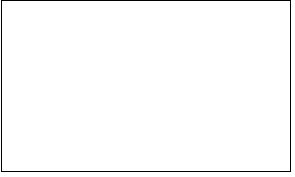
\includegraphics{figs/grabs.pdf}
\end{graphicalabstract}

\begin{highlights}
\item Research highlights item 1
\item Research highlights item 2
\item Research highlights item 3
\end{highlights}

\begin{keywords}
 \sep \AMOC \sep  \sep 
\end{keywords}

\maketitle


\section{Introduction}

A simple linear regression representing the AMOC as a single-layer dynamic model showed that the western boundary temperature anomaly at 400 decibar (dbar) explained 53\% of the variance in the transport anomaly of the thermocline (0-800 m) layer \citep{longworth2011}.

\section{Materials and methods}

We repeated the simple linear regression from \citet{longworth2011} using monthly mean temperatures from the RAPID western boundary moorings instead of CTD data. Despite the resulting regression having almost identical slope and intercept, we found that it explained only 10\% of the variance of the thermocline layer transport, rather than 53\% as \citet{longworth2011} found. Concluding that representing a single layer did not sufficiently explain the AMOC dynamics at 26\textdegree N, we investigated representing two, three and four layers: first with boundary temperature and salinity anomalies; and then with boundary density anomalies.

- creation of model

- dynamic relationship

- justification of using a linear regression model?

- testing of model

- cross-validation?

- testing against RAPID

- evaluating uncertainty - Monte Carlo method/bootstrapping

- prediction intervals

- model assumptions - autocorrelation of residuals, non-stationarity of variables

- types of model - OLS, GLSAR, ARIMA, SARIMAX?


The model was created using data from the RAPID project from ?? Apr 2004 to ?? ?? 2017. To create dynamic height profiles to calculate geostrophic transport across the basin, several moorings on both western and eastern boundaries are combined to make single full height profiles of temperature and salinity, interpolated over a 20 dbar grid. The full method is detailed in \cite{mccarthy2015}. Data from a subsequent RAPID cruise was used to test the model against RAPID's own MOC estimate.

The historical hydrographic data came from multiple sources: the Western Boundary Time Series (WBTS); the underlying profiles used to create the Met Office EN4 reanalysis; the World Ocean Database (WOD); TODO.

- issues with using reanalysis data, i.e., no real deep (4100 dbar) data

%\section{Theory/calculation}

\section{Results}

-- transatlantic section data

-- en4 data

-- other hydrographic data

-- 

\section{Discussion}

\section{Conclusion}

\section{Acknowledgements}

\section{Funding}

This work was supported by the Natural Environmental Research Council [grant number NE/L002531/1]



 

\begin{figure}
	\centering
		
\includegraphics[scale=.75]{figs/Fig1.pdf}
	\caption{The evanescent light - $1S$ quadrupole coupling
	($g_{1,l}$) scaled to the bulk exciton-photon coupling
	($g_{1,2}$). The size parameter $kr_{0}$ is denoted as $x$ and
	the \PMS is placed directly on the cuprous oxide sample ($\delta
	r=0$, See also Table \protect\ref{tbl1}).}
	\label{FIG:1}
\end{figure}



\begin{table}[width=.9\linewidth,cols=4,pos=h]
\caption{This is a test caption. This is a test caption. This is a test
caption. This is a test caption.}\label{tbl1}
\begin{tabular*}{\tblwidth}{@{} LLLL@{} }
\toprule
Col 1 & Col 2 & Col 3 & Col4\\
\midrule
12345 & 12345 & 123 & 12345 \\
12345 & 12345 & 123 & 12345 \\
12345 & 12345 & 123 & 12345 \\
12345 & 12345 & 123 & 12345 \\
12345 & 12345 & 123 & 12345 \\
\bottomrule
\end{tabular*}
\end{table}



\appendix
\section{My Appendix}
Appendix sections are coded under \verb+\appendix+.

\verb+\printcredits+ command is used after appendix sections to list 
author credit taxonomy contribution roles tagged using \verb+\credit+ 
in frontmatter.

\printcredits

%% Loading bibliography style file
%\bibliographystyle{model1-num-names}
\bibliographystyle{cas-model2-names}

% Loading bibliography database
\bibliography{../../OneDrive/PhD/References/simplified_model}


%\vskip3pt

%\bio{}
%Author biography without author photo.
%Author biography. Author biography. Author biography.
%Author biography. Author biography. Author biography.
%Author biography. Author biography. Author biography.
%Author biography. Author biography. Author biography.
%Author biography. Author biography. Author biography.
%Author biography. Author biography. Author biography.
%Author biography. Author biography. Author biography.
%Author biography. Author biography. Author biography.
%Author biography. Author biography. Author biography.
%\endbio
%
%\bio{figs/pic1}
%Author biography with author photo.
%Author biography. Author biography. Author biography.
%Author biography. Author biography. Author biography.
%Author biography. Author biography. Author biography.
%Author biography. Author biography. Author biography.
%Author biography. Author biography. Author biography.
%Author biography. Author biography. Author biography.
%Author biography. Author biography. Author biography.
%Author biography. Author biography. Author biography.
%Author biography. Author biography. Author biography.
%\endbio
%
%\bio{figs/pic1}
%Author biography with author photo.
%Author biography. Author biography. Author biography.
%Author biography. Author biography. Author biography.
%Author biography. Author biography. Author biography.
%Author biography. Author biography. Author biography.
%\endbio


\end{document}

